\documentclass[11pt]{article}

\usepackage[margin=1in]{geometry}
\usepackage{times}
\usepackage{booktabs}
\usepackage{multirow}
\usepackage{amsmath}
\usepackage[colorlinks=true,linkcolor=blue,citecolor=blue,urlcolor=blue]{hyperref}
\usepackage{xcolor}
\usepackage{graphicx}
\usepackage{natbib}
\usepackage{tikz}
\usetikzlibrary{positioning,arrows.meta,shapes.geometric}

\newcommand{\todo}[1]{\textcolor{red}{\textbf{[TODO: #1]}}}
\newcommand{\pending}[1]{\textcolor{orange}{\textbf{[PENDING: #1]}}}

\title{Bounded Structural Primitives versus Generic Tool Use\\
for Agentic Word Document Editing: A Confirmatory Benchmark}

\author{Adam Camerer \\ \todo{affiliation}}

\date{Preliminary draft --- \today}

\begin{document}
\maketitle

\begin{abstract}
Many agent systems increasingly edit real documents through generic file-manipulation tools
(read, write, search-and-replace, shell commands) rather than through primitives designed for
the document's own format. On the same model and the same documents, we ask whether Meridian
Docs' document-editing tools -- a bounded, atomic, structurally-aware subset of that package's
much larger MCP tool surface (Section~\ref{sec:limitations}), for Microsoft Word's Office Open
XML (OOXML/\texttt{.docx}) format -- change task correctness relative to an
agent given only generic tools and raw XML access. We report a confirmatory benchmark across six task families
(bibliography-entry insertion, inline citation insertion, section reordering, equation insertion,
table-structural insertion, and figure-caption insertion) on a held-out corpus of real, previously
unseen \texttt{.docx} documents, each task run as a forward edit followed by its own inverse and
independently graded against the original document's structure. Two families
(bibliography, citation) show no measurable difference between arms. One family (section
reordering) shows no difference on a single edit but a statistically significant advantage for
the bounded tool under four repeated edit-undo cycles (92.9\% vs.\ 67.3\% pass rate, $p=0.0015$),
traced to a specific, data-grounded failure mode in the generic-tool arm: compounding loss of
the true original document state across repeated cycles, a pattern consistent with \emph{state
drift} as described in agentic-LLM settings \citep{wu2026dualanchoring}. Three families (equation, table-structural, and caption insertion) share a
write-time structural-correctness verification step; on a shared, variably-contended host, two of
the three reported markedly lower pass rates (equation 46.2\%, caption 7.7\%) while table-structural
reached 96.2\%. We treated this as a hypothesis rather than a finding and tested it directly: a
controlled, isolated timing test first rejected task-dependent render cost as the explanation,
and a full confirmatory re-run of the identical benchmark -- same model, same corpus, same
code -- on a dedicated, single-tenant cloud host closed the gap completely, all three families
reaching 100\% pass for both arms. The original numbers were a deployment-environment artifact
(shared-host scheduling contention, a physically unreliable storage device, and confirmed network
failures), not an editing-capability limitation, and we report both the original and the
confirmatory numbers rather than replacing one with the other silently. Separately, we
document ten
infrastructure and evaluation-harness defects that this benchmark's own development surfaced and
fixed -- several of which materially changed the reported numbers -- disclosed in full rather
than silently corrected.
\end{abstract}

\section{Introduction}
\label{sec:intro}

When agents use large language models to edit real documents -- inserting a citation, reordering
a section, adding a table -- they typically do so one of two ways. In the first, the agent is
given generic file tools (read a file, write a file, run a shell command) and is expected to
construct or edit the document's own serialization format correctly by direct manipulation, the
same way a human would edit raw markup in a text editor. In the second, the agent is given a
small number of purpose-built, bounded operations -- \emph{insert this table here},
\emph{remove this citation} -- that internally guarantee the document remains structurally
valid.

The second approach is a common design pattern in tool-augmented agent systems generally: it
underlies benchmarks in software engineering (SWE-bench), open-web navigation (WebArena), and
general-purpose tool use (GAIA) alike \citep{jimenez2023swebench,zhou2024webarena,mialon2023gaia}
-- each of which measures whether an agent completes a task under one fixed tool surface, not
whether the shape of that surface itself changes the outcome. For document editing specifically,
that tradeoff is under-characterized: bounded tools cost engineering effort to build and
constrain what an agent can express, while generic tools cost nothing to provide but ask the
model to get low-level format details right on every call, with no structural safety net.
Getting this wrong is costly in different directions: bounded tools that prove unnecessary waste
engineering effort, while generic tools that seem fine on a single edit may fail silently as an
agent keeps working on the same document over time. This paper reports a confirmatory, paired
benchmark designed to measure that tradeoff directly, for one concrete document format
(Microsoft Word's \texttt{.docx}, standardized as Office Open XML \citep{ecma376}) and one
concrete set of editing tasks.

\subsection{Research questions}
\label{sec:rqs}
Three questions were fixed before any trial in this paper was run (Section~\ref{sec:methods}'s
preregistration commit hashes), and each maps directly to one of this paper's three main
results:
\begin{description}
\item[RQ1] On a single forward/inverse edit, does a bounded tool pair change task correctness
  relative to generic tools, for each of six document-editing task families? (Table~\ref{tab:single-edit},
  Table~\ref{tab:render-gate-clean})
\item[RQ2] Under four repeated edit-undo cycles on the same document, does either arm's
  correctness compound or decay with repetition? (Section~\ref{sec:section-reorder},
  Table~\ref{tab:k4})
\item[RQ3] If a write-time structural-verification step produces a large gap between arms, is
  that gap attributable to the editing operations themselves or to the deployment environment
  they were measured in? (Section~\ref{sec:render-gate}, Section~\ref{sec:methods-rerun})
\end{description}
RQ3 was not itself preregistered -- it is a post-hoc question motivated by an anomaly RQ1's own
data revealed (Section~\ref{sec:render-gate}) -- and we report it as a diagnostic investigation
of that anomaly, not as a fourth planned confirmatory test on equal footing with RQ1/RQ2.

\subsection{Design}

Each of six task families is defined as a \emph{forward} edit (e.g., insert a bibliography
entry) and its own \emph{inverse} (remove that same entry), run in sequence against the same
document, so that a correct round trip leaves the document's original content unchanged. Every
task is run twice on the same starting document under the same model: once with a \textbf{control}
arm restricted to generic \texttt{Read}/\texttt{Write}/\texttt{Edit}/\texttt{Bash} tools and
direct access to the document's raw XML, and once with a \textbf{treatment} arm restricted to
exactly one bounded, purpose-built tool pair for that family and no generic editing tools at
all. Both arms use the same underlying language model (\texttt{claude-sonnet-5}); the only
manipulated variable is which tool surface the agent can act through. Grading (Section~\ref{sec:methods})
is performed entirely outside the agent, never by trusting its own transcript claim of success.

\subsection{Contributions}

\begin{itemize}
\item We present a confirmatory, paired benchmark across six real document-editing task
  families, on a held-out corpus never used during the tooling's own development
  (Section~\ref{sec:results}), with per-family sample sizes and paired significance tests
  reported honestly, including families where the two arms show no measurable difference.
\item We demonstrate that bounded structural tools show no advantage on a single edit but a
  significant advantage under repeated edit-undo cycling, and identify the mechanism: the
  generic-tool arm's correctness degrades with repetition (state drift) while the bounded
  tool's does not (Section~\ref{sec:section-reorder}).
\item We identify a confound introduced by a write-time structural-verification step shared by
  three of the six families, and resolve it with a controlled confirmatory re-run of the
  identical benchmark on a dedicated, single-tenant host, which closes the gap completely and
  confirms the confound was a deployment-environment artifact, not a capability limitation
  (Section~\ref{sec:render-gate}).
\item We disclose ten infrastructure, harness, and evaluation-code defects found during this
  project -- each with its root cause, fix, and independent re-verification -- and show that
  several materially changed an already-reported number (Section~\ref{sec:defects}).
\end{itemize}

\section{Related Work}
\label{sec:related}

Benchmarks for tool-augmented and agentic LLM behavior have largely targeted software
engineering \citep{jimenez2023swebench}, open-ended web navigation \citep{zhou2024webarena}, and
general-purpose real-world task completion requiring tool use and multi-step reasoning
\citep{mialon2023gaia}. These benchmarks measure whether an agent \emph{can accomplish} a task
given some fixed tool surface; they do not hold the underlying task and model fixed while
varying only the shape of that tool surface (bounded versus generic) as the manipulated
variable, which is the specific question this paper addresses for one document-editing domain.

A separate line of work studies whether constraining an LLM's \emph{output format} changes its
performance, rather than whether the \emph{tool surface itself} is bounded or generic:
\citet{tam2024letmespeak} find that structured-format restrictions (JSON, XML) measurably degrade
LLM reasoning relative to free-form generation, and \citet{patil2023gorilla} show that grounding
tool calls in a fixed, retrieval-aware API surface reduces call-hallucination. Both manipulate the
shape of the model's own output; this paper instead holds output format fixed (a real \texttt{.docx}
file either way) and manipulates which tools can produce it. For document-format-aware editing
specifically, the closest prior work targets sibling Office Open XML formats rather than Word
directly: \citet{li2023sheetcopilot} give an LLM a bounded set of atomic spreadsheet actions, and
\citet{ofengenden2025pptarena} evaluate an agent that routes between programmatic tools and
deterministic XML operations for PowerPoint editing, verifying each edit before committing it --
an architecture directly analogous to Meridian Docs' own write-time verification
(Section~\ref{sec:render-gate}), applied to a different OOXML-based format. We are not aware of
prior work posing this paper's specific bounded-versus-generic comparison for Word/OOXML editing
itself.

\section{Methods}
\label{sec:methods}

\subsection{Corpus}
The primary corpus is a 26-document, previously licensed and audited slice of the DocOps
benchmark corpus (real, unmodified business records such as internal memos, written policies,
and meeting minutes, not hand-authored fixtures), split into a 14-document primary holdout and a
12-document validation set, pooled into the flat $n=26$ reported throughout this paper. This
corpus's own construction is independently preregistered, prior to any trial reported
here.\footnote{2026-08-27, commit \texttt{1061e0e}, this project's evaluation-harness repository.}
Neither subset was used to design the tooling's original feature set, but several defects
(Section~\ref{sec:defects}) were subsequently found by observing this corpus's own trial outcomes
during the benchmark's execution and fixed directly in the tooling, with every affected chain then
independently re-run and re-graded rather than assumed fixed. We disclose this iterative
debug-and-rerun cycle in full (Section~\ref{sec:defects}, Section~\ref{sec:limitations}) rather
than describe either subset as a blind holdout in the machine-learning sense -- it is not one. A
separately preregistered (2026-08-31, \texttt{e813cd7}) 48-document follow-up corpus was built
specifically for the section-reordering family, because the primary corpus yields only 11
documents on which that task is structurally applicable; the follow-up corpus itself yields 44
applicable documents (of 48), so the combined section-reordering corpus reported in
Table~\ref{tab:single-edit} and Table~\ref{tab:k4} is $11+44=55$ paired documents, not
$11+48=59$.

\subsection{Task families}
Six families are reported, each implemented as one forward/inverse tool pair in Meridian Docs on
the treatment side:
\begin{itemize}
\item \textbf{Bibliography entry} -- insert/remove one APA-formatted bibliography entry.
\item \textbf{Inline citation} -- insert/remove one inline citation marker.
\item \textbf{Section reorder} -- move a section after a different heading, then move it
  back.\footnote{The destination heading is validated at two layers: \texttt{move\_section}
  rejects any destination whose index falls inside the moved section's own body range (bounded by
  the next heading at the same or shallower level), so a heading that is structurally a child of
  the section being moved is always refused; the benchmark's own destination-picker independently
  requires a same-or-shallower-level heading when constructing each trial, so that case is never
  even proposed to either arm.}
\item \textbf{Equation} -- insert/remove one native OOXML math object (\texttt{<m:oMath>}), not
  plain text formatted to resemble an equation.\footnote{A separate, unmerged prototype for
  LaTeX-OMML round-trip fidelity and notation-style auditing exists for a different,
  journal-specific conversion use case; it shares no code with the tool exercised here and is out
  of scope for this benchmark.}
\item \textbf{Table (structural)} -- insert/remove one whole Word table (a real
  \texttt{<w:tbl>} object with genuine rows and columns), not text formatted to look tabular.
\item \textbf{Caption} -- insert/remove one numbered SEQ-field figure caption.
\end{itemize}

\begin{figure}[h]
\centering
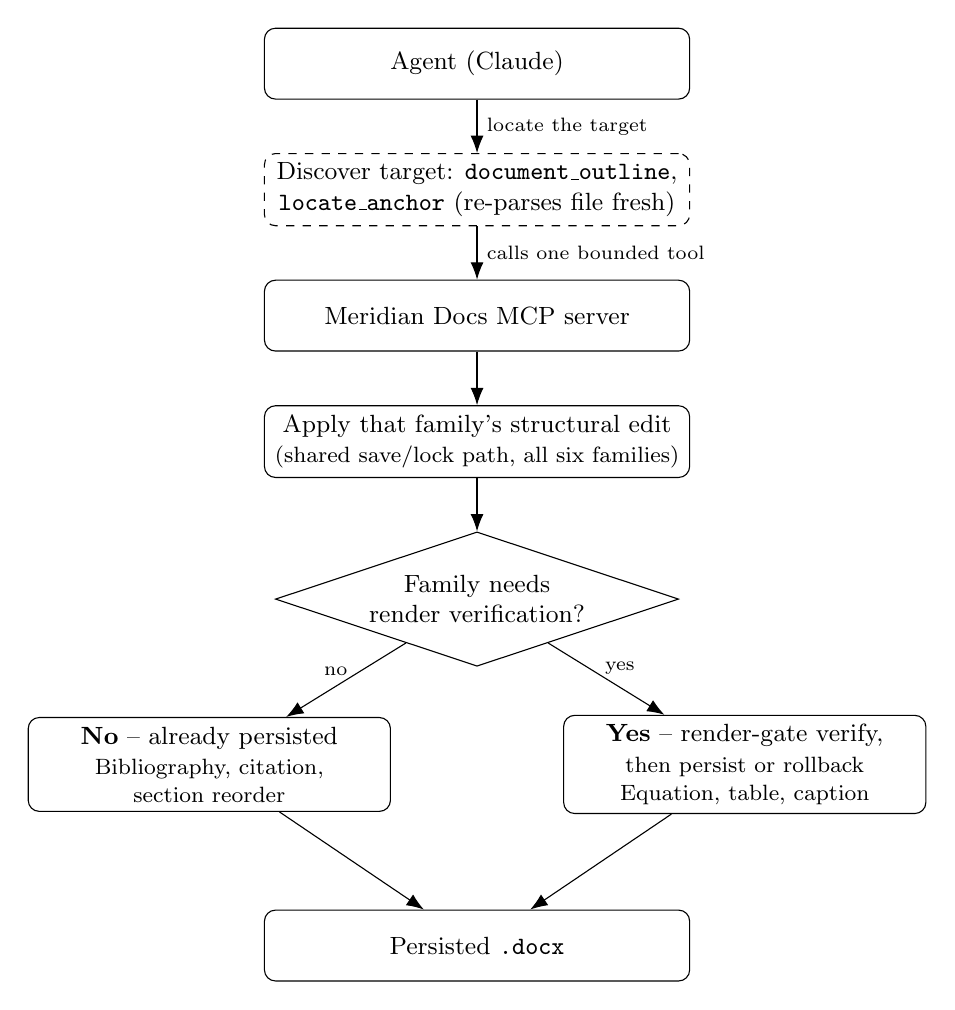
\begin{tikzpicture}[
  box/.style={draw, rounded corners, align=center, minimum height=0.9cm, minimum width=5.4cm, font=\small},
  dbox/.style={draw, dashed, rounded corners, align=center, minimum height=0.9cm, minimum width=5.4cm, font=\small},
  decision/.style={draw, diamond, aspect=3, align=center, font=\small, inner sep=2pt},
  branch/.style={draw, rounded corners, align=center, minimum height=1.05cm, minimum width=4.6cm, font=\small},
  arr/.style={-{Latex[length=2.2mm]}},
  lbl/.style={font=\scriptsize}
]
\node[box] (agent) at (0, 10.4) {Agent (Claude)};
\node[dbox] (discover) at (0, 8.8) {Discover target: \texttt{document\_outline},\\\texttt{locate\_anchor} (re-parses file fresh)};
\node[box] (mcp) at (0, 7.2) {Meridian Docs MCP server};
\node[box] (edit) at (0, 5.6) {Apply that family's structural edit\\\footnotesize (shared save/lock path, all six families)};
\node[decision] (needsgate) at (0, 3.6) {Family needs\\render verification?};

\node[branch] (direct) at (-3.4, 1.5)
  {\textbf{No} -- already persisted\\
   \footnotesize Bibliography, citation,\\[-1pt]
   \footnotesize section reorder};
\node[branch] (gated) at (3.4, 1.5)
  {\textbf{Yes} -- render-gate verify,\\
   \footnotesize then persist or rollback\\[-1pt]
   \footnotesize Equation, table, caption};

\node[box] (docx) at (0, -0.8) {Persisted \texttt{.docx}};

\draw[arr] (agent) -- node[lbl, right] {locate the target} (discover);
\draw[arr] (discover) -- node[lbl, right] {calls one bounded tool} (mcp);
\draw[arr] (mcp) -- (edit);
\draw[arr] (edit) -- (needsgate);
\draw[arr] (needsgate) -- node[lbl, above left=-2pt and -4pt] {no} (direct);
\draw[arr] (needsgate) -- node[lbl, above right=-2pt and -4pt] {yes} (gated);
\draw[arr] (direct) -- (docx);
\draw[arr] (gated) -- (docx);
\end{tikzpicture}
\caption{Meridian Docs' overall functional architecture, including the discovery step a real
deployment needs (this benchmark's harness bypasses it -- Section~\ref{sec:methods}). Editing
itself is a shared step for all six families; render-gate verification is a sequential,
conditional step layered on \emph{after} the edit, only for the three structural families,
detailed in Figure~\ref{fig:rendergate-arch} -- not an independent alternative path chosen from
the start. This split is exactly the property that Section~\ref{sec:render-gate} shows produces
markedly different reliability behavior.}
\label{fig:architecture}
\end{figure}

\subsection{Arms and isolation}
The control arm receives \texttt{Read}, \texttt{Write}, \texttt{Edit}, and \texttt{Bash}, with
no access to any purpose-built document-editing tool. The treatment arm receives exactly one
bounded tool pair and \texttt{Read}, with no generic write access at all -- for the
table-structural family, for example, \texttt{insert\_table} and \texttt{remove\_table}. We
post-hoc audited every trial's transcript for isolation
violations -- a control transcript referencing a purpose-built tool name, or a treatment
transcript referencing any tool outside its one declared pair, would indicate a harness leak --
and found no such violation in any reported trial. Neither arm's tool set includes a
structure-discovery tool (e.g., \texttt{locate\_anchor}, \texttt{document\_outline}): the target
anchor for each forward edit is resolved once, at corpus-build time, and supplied directly in the
trial's prompt, so indexing/discovery-tool availability is not part of what this benchmark
measures -- only editing correctness given a target that is already known.

Discovery and editing share the same tool surface deliberately, not incidentally:
\texttt{locate\_anchor} and \texttt{document\_outline} return the same identifier format
(\texttt{w14:paraId}, or a content-derived fallback for paragraphs without one) that the editing
tools themselves accept as a target, so a call to one composes directly with a call to the
other. Leaving discovery to the agent's own reading instead, as the control arm does, means
locating a target by prose/structural interpretation rather than by a structurally valid id --
exactly the fragile targeting this benchmark's state-drift finding
(Figure~\ref{fig:drift-mechanism}) traces the control arm's failures to. Nor does staying correct
across edits require any scheduled reindexing: \texttt{locate\_anchor} keeps no persistent index
at all, re-parsing the live file fresh on every call, and the native \texttt{w14:paraId}
identifier itself is not an externally-maintained index but an attribute OOXML stores directly on
each paragraph, persisting automatically through ordinary saves. A separate part of Meridian
Docs, \texttt{index\_document}, does maintain a persisted index for broader search/outline
features outside this benchmark's scope; it handles staleness by content-hash/mtime detection
that fails closed on a mismatch, not a fixed reindexing schedule.

\subsection{Grading}
We graded every trial's output \texttt{.docx} independently of the agent's own report, by
parsing the file's actual XML after the trial completed: the forward direction graded pass only
if the expected content was present exactly once and every pre-existing paragraph was unchanged;
the inverse direction graded pass only if that content was fully removed and the document's
paragraph list exactly matched its pre-forward state. A chain (one forward/inverse pair) counted
as a full pass only if both directions independently graded pass.

\subsection{Statistics}
Per-family pass rates are reported with percentile bootstrap confidence intervals (2{,}000
resamples) \citep{efron1979bootstrap}, except at a literal 100\% or 0\% observed rate, where the
percentile method is degenerate (every possible resample is identical to the original sample) and
we report the exact Clopper-Pearson interval instead (Section~\ref{sec:defects}, defect 9). Paired
arms are compared with a paired sign-flip
permutation test (2{,}000 resamples) \citep{nichols2002permutation}, with a fixed random seed
set before any result existed. We report every comparison this benchmark's design specifies (six
families, at $K=1$, plus the one preregistered $K=4$ depth study) rather than a subset, and do
not apply a multiple-comparison correction across them: the $K=4$ section-reorder result is the
one comparison this benchmark's design was built in advance to make (Section~\ref{sec:section-reorder}),
not one significant finding selected after the fact from many equally-likely candidates, so we
report it and its p-value directly rather than adjusting it for tests it was never in competition
with. A chain that never executed or never finished because of a
harness- or infrastructure-level failure unrelated to the task itself (a network error, a
process-level subprocess timeout) is excluded from both arms' denominators for that document,
rather than scored as a failure. This per-trial subprocess timeout is 300 seconds (600 seconds for
the render-gated families, Section~\ref{sec:defects} defect 7); neither value was derived from an
expected-task-duration analysis -- 300s was an uninstrumented initial choice and 600s a reactive
doubling to survive a specific host-contention episode -- which we note as a limitation
(Section~\ref{sec:limitations}) rather than a principled budget. A chain that executed to completion and reports a genuine
task-level failure -- including a write-time structural-verification failure under host
contention (Section~\ref{sec:render-gate}), since that is a property of the treatment condition
being measured, not an unrelated infrastructure artifact -- is scored as a failure at a fixed
denominator. The one repeated-cycling ($K=4$) design compares steady-state pass rate (the
fraction of chains passing every one of the four cycles) across four consecutive forward/inverse
cycles on the same document, rather than a single cycle, specifically to test whether either
arm's correctness compounds or decays under repetition.

\subsection{Confirmatory re-run environment}
\label{sec:methods-rerun}
The three write-time-verification-gated families (Section~\ref{sec:render-gate}) were originally
run on a shared Windows host also used for other concurrent work, and their pass rates were
markedly lower for two of the three. To test whether that reflected the editing operations
themselves or the host, we re-ran the identical benchmark -- unchanged model, corpus, harness,
and grading code -- on a dedicated, single-tenant cloud CPU instance (4 dedicated vCPUs, no other
tenant or process competing for the same physical resources). Two environment differences were
necessary and are disclosed here rather than left implicit. First, the instance runs Linux, so
the write-time verification step's Microsoft Word COM backend (Windows-only) is unavailable; only
its LibreOffice/\texttt{soffice} backend runs. This does not change what is being measured: an
audit of every persisted chain result across the original host's full run history found the
Word COM backend never won the two-backend race on its own in any recorded successful chain (it
only ever appears in failure records where both backends failed together), so a
LibreOffice-only environment is evaluating the same effective verification path the original run
already relied on almost exclusively, not a different one. Second, the CLI executing each trial
refuses to run with permission checks bypassed when invoked as the root user, a restriction the
original host (a non-root desktop account) never triggered; we created a dedicated non-root
account on the instance for this reason, verified functionally, and re-ran the affected trials
that had failed instantly under root before this was found.

\section{Results}
\label{sec:results}

\subsection{Single-edit families}
\label{sec:single-edit}

\begin{table}[h]
\centering
\begin{tabular}{lccccc}
\toprule
Family & Arm & Pass rate & 95\% CI & $n$ & Paired $p$ \\
\midrule
Bibliography entry & control   & 100\% & [86.8, 100]$^\dagger$ & 26 & \multirow{2}{*}{1.0} \\
                    & treatment & 100\% & [86.8, 100]$^\dagger$ & 26 & \\
\addlinespace
Inline citation\footnote{Treatment $n=25$: one forward call hit a genuine 300-second
process-level subprocess timeout unrelated to the citation task itself, excluded from the
denominator per Section~\ref{sec:methods}'s harness-flake rule rather than scored as a
failure.} & control   & 100\% & [86.8, 100]$^\dagger$ & 26 & \multirow{2}{*}{1.0} \\
                    & treatment & 100\% & [86.3, 100]$^\dagger$ & 25 & \\
\addlinespace
Section reorder (original corpus) & control   & 72.7\% & [45.5, 100]  & 11 & \multirow{2}{*}{0.240} \\
                                   & treatment & 100\%  & [71.5, 100]$^\dagger$   & 11 & \\
\addlinespace
Section reorder (combined, v1+v2)\footnote{Control $n=55$, treatment $n=56$: one 1.7MB document's
control-arm chain never completed within the harness's 300-second timeout across six independent
attempts at varying host load (a real, document-size-driven control-arm limitation, excluded
from control's denominator only), while its treatment-arm chain completed and passed.} & control   & 83.6\% & [74.5, 92.7] & 55 & \multirow{2}{*}{0.271} \\
                                       & treatment & 92.9\% & [85.7, 98.2] & 56 & \\
\bottomrule
\end{tabular}
\caption{Single-edit ($K=1$) results for the four families not gated by write-time
structural-verification. Bibliography and citation show a genuine, literal parity between arms.
Section reorder shows a directionally consistent but not-yet-significant advantage for the
bounded tool at $K=1$; see Section~\ref{sec:section-reorder} for the $K=4$ result on the same
corpus. $^\dagger$Exact Clopper-Pearson interval rather than the percentile bootstrap used
elsewhere (Section~\ref{sec:defects}, defect 9): at a literal 100\% observed rate every possible
bootstrap resample is identical to the original sample, so the percentile method itself cannot
express any uncertainty there.}
\label{tab:single-edit}
\end{table}

Table~\ref{tab:single-edit} shows bibliography and citation with no measurable difference
between arms at any sample size tested: both reached a literal 100\%/100\% parity once two real
evaluation-harness defects (described in Section~\ref{sec:defects}) were found and fixed.
Section reordering's original 11-document result looked directionally favorable to the bounded
tool but was underpowered
($p=0.240$); a larger, independently preregistered 48-document follow-up corpus, combined with
the original, narrowed but did not close that gap at $K=1$ ($p=0.271$).

\subsection{Repeated cycling: the one significant finding}
\label{sec:section-reorder}

\begin{table}[h]
\centering
\begin{tabular}{lccccc}
\toprule
Family & Arm & Pass rate & 95\% CI & $n$ & Paired $p$ \\
\midrule
Section reorder ($K=4$, combined) & control   & 67.3\% & [54.5, 78.2] & 55 & \multirow{2}{*}{\textbf{0.0015}} \\
                                   & treatment & 92.9\% & [85.7, 98.2] & 56 & \\
\bottomrule
\end{tabular}
\caption{Under four repeated edit-undo cycles, the bounded tool holds a 92.9\% pass rate while
the generic tool falls to 67.3\% ($p=0.0015$). Same combined corpus as Table~\ref{tab:single-edit}'s
bottom row.}
\label{tab:k4}
\end{table}

Run through four repeated edit-undo cycles rather than one, the same 55/56-document combined
corpus produced the single significant result in this benchmark (Table~\ref{tab:k4}): control's
pass rate fell to 67.3\% while treatment held at 92.9\% ($p=0.0015$). This is not a p-value
found by fishing
across many cuts of the data -- it is the specific comparison the $K$-sweep design was built to
make, on the same corpus already reported at $K=1$.

The mechanism was traced directly rather than inferred from the p-value alone, in the
48-document v2 follow-up sub-corpus specifically (the source of the finer per-cycle grading
breakdown below; the full 55/56 combined corpus is not broken down at this granularity in this
draft). Of the 12 v2-corpus control chains with at least one failing cycle, 9 failed specifically
on exact-order restoration starting from the second cycle onward -- a real, dominant majority
pattern, not a universal rule -- and 2 failed that same check on the very first cycle (one of
those two then recovering fully on later cycles); the remaining chain's specific failure
category is not itemized in our current evidence record, a gap we disclose rather than paper
over. The bounded tool showed no equivalent drift on
any chain, in either sub-corpus. This is consistent
with a specific, plausible cause: the bounded tool re-resolves a fresh structural anchor for the
target section on every call, while the generic-tool agent must reconstruct or remember ``the
original layout'' itself across calls, and that reconstruction compounds error with repetition.
The pattern is dominant but not exceptionless (2 of 12 control failures occur on the very first
cycle, one of those two then recovering on a later cycle) -- the significance finding rests on
the dominant trend, not on every case fitting the same story.

\begin{figure}[h]
\centering
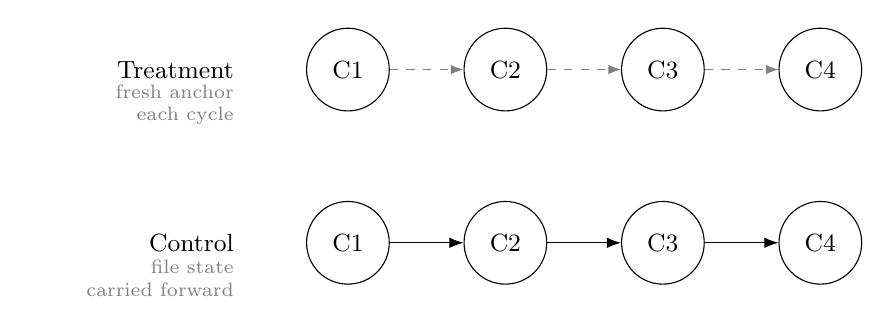
\begin{tikzpicture}[
  cyc/.style={draw, circle, minimum size=1.05cm, font=\small},
  rowlab/.style={font=\small, align=right, text width=2.5cm},
  sublab/.style={font=\scriptsize, align=right, text width=2.5cm, text=gray},
  arr/.style={-{Latex[length=1.8mm]}},
  timearr/.style={-{Latex[length=1.6mm]}, gray, dashed},
]
\node[rowlab] (tlabel) at (-2.2, 2.2) {Treatment};
\node[sublab] (tsub) at (-2.2, 1.75) {fresh anchor\\each cycle};
\node[cyc] (t1) at (0.5, 2.2) {C1};
\node[cyc] (t2) at (2.5, 2.2) {C2};
\node[cyc] (t3) at (4.5, 2.2) {C3};
\node[cyc] (t4) at (6.5, 2.2) {C4};
\draw[timearr] (t1) -- (t2);
\draw[timearr] (t2) -- (t3);
\draw[timearr] (t3) -- (t4);

\node[rowlab] (clabel) at (-2.2, 0) {Control};
\node[sublab] (csub) at (-2.2, -0.45) {file state\\carried forward};
\node[cyc] (c1) at (0.5, 0) {C1};
\node[cyc] (c2) at (2.5, 0) {C2};
\node[cyc] (c3) at (4.5, 0) {C3};
\node[cyc] (c4) at (6.5, 0) {C4};
\draw[arr] (c1) -- (c2);
\draw[arr] (c2) -- (c3);
\draw[arr] (c3) -- (c4);
\end{tikzpicture}
\caption{The mechanism behind Table~\ref{tab:k4}'s result. Treatment re-resolves its target by
a stable structural id fresh each cycle (dashed: no real dependency between cycles). Control has
no such anchor, so each cycle's unverified edit builds on whatever the previous cycle actually
left in the file (solid: a real dependency an undetected mistake can cross).}
\label{fig:drift-mechanism}
\end{figure}

\begin{figure}[h]
\centering
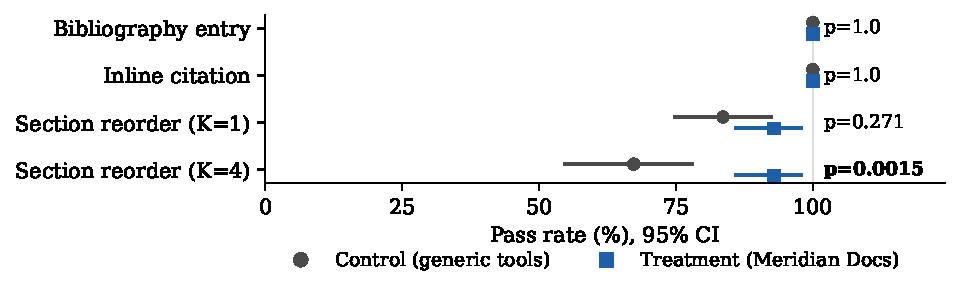
\includegraphics[width=0.85\textwidth]{figures/fig-single-edit-forest.pdf}
\caption{Pass rate and 95\% CI by arm for the four families not gated by write-time
structural-verification (Table~\ref{tab:single-edit}, Table~\ref{tab:k4}). Bibliography and
citation show literal overlap; section reorder's confidence intervals narrow but still overlap at
$K=1$ and separate cleanly at $K=4$, the benchmark's one significant single-family comparison.}
\label{fig:single-edit}
\end{figure}

Figure~\ref{fig:single-edit} shows this pattern directly: three of the four comparisons show
near-total overlap between arms, while section reorder's confidence intervals separate cleanly
only once cycling reaches $K=4$.

\subsection{Write-time structurally-verified families}
\label{sec:render-gate}

The remaining three families (equation, table, caption) share one architectural property the
first four do not: their treatment-side insertion tool verifies its own write correctness before
persisting a change -- rendering the resulting document with an independent renderer and
confirming it opens without error -- and it atomically restores the original file if that
verification fails for any reason. This design choice trades a real reliability cost
(verification against a real renderer is slow, and slower still on a resource-contended host)
for a strong guarantee: a persisted change from these three tools is, by construction, never a
corrupt or unopenable document.

This split tracks OOXML synthesis risk, not edit importance: equation, table, and caption
insertion each construct a brand-new, schema-fragile structure from scratch -- a foreign-namespace
\texttt{<m:oMath>} tree, a \texttt{<w:tbl>} grid whose child element order OOXML validates
strictly, or a SEQ-numbered field wrapped in a document-unique bookmark pair -- where a structural
re-parse can confirm the result is well-formed XML but not that Word will actually open it.
Bibliography and citation insertion instead append or create only plain runs or an
already-proven complex-field idiom onto an already-valid paragraph, and section reordering
relocates already-valid elements without synthesizing any new XML shape at all: none of the other
three families introduces a genuinely novel structural risk, so they are gated with structural
verification alone, or not at all, rather than paying render-gate's latency cost.

\begin{figure}[h]
\centering
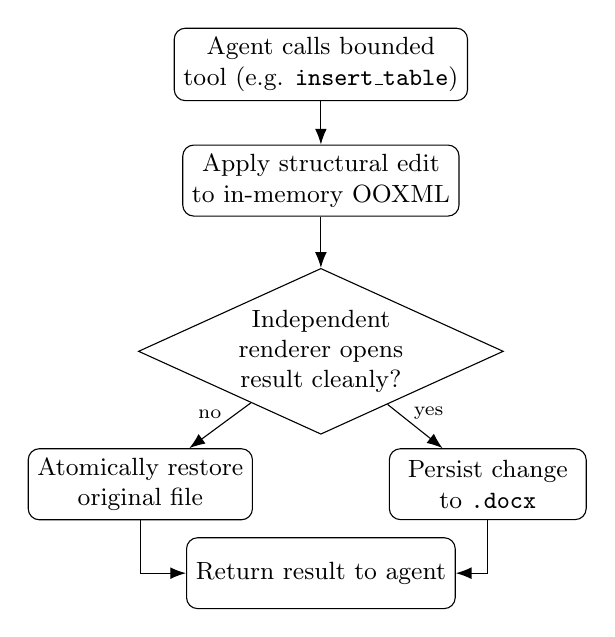
\begin{tikzpicture}[
  node distance=0.55cm and 1.0cm,
  box/.style={draw, rounded corners, align=center, minimum height=0.9cm, minimum width=2.5cm, font=\small},
  decision/.style={draw, diamond, aspect=2.2, align=center, font=\small, inner sep=1pt},
  arr/.style={-{Latex[length=2mm]}},
  lbl/.style={font=\scriptsize, midway}
]
\node[box] (call) {Agent calls bounded\\tool (e.g. \texttt{insert\_table})};
\node[box, below=of call] (edit) {Apply structural edit\\to in-memory OOXML};
\node[decision, below=0.65cm of edit] (verify) {Independent\\renderer opens\\result cleanly?};
\node[box, below left=0.7cm and -0.3cm of verify] (fail) {Atomically restore\\original file};
\node[box, below right=0.7cm and -0.3cm of verify] (ok) {Persist change\\to \texttt{.docx}};
\node[box, below=1.3cm of verify] (ret) {Return result to agent};

\draw[arr] (call) -- (edit);
\draw[arr] (edit) -- (verify);
\draw[arr] (verify) -- node[lbl, above left=-1pt and -4pt] {no} (fail);
\draw[arr] (verify) -- node[lbl, above right=-1pt and -4pt] {yes} (ok);
\draw[arr] (fail) |- (ret);
\draw[arr] (ok) |- (ret);
\end{tikzpicture}
\caption{Meridian Docs' write-time verification flow, shared by the equation, table-structural,
and caption insertion tools (Section~\ref{sec:render-gate}). Control-arm edits bypass this path
entirely -- they write raw XML directly, with no independent render-verification step.}
\label{fig:rendergate-arch}
\end{figure}

Figure~\ref{fig:rendergate-arch} shows this flow. The verification step itself races two
independent renderer backends concurrently (Section~\ref{sec:defects}, defect 7) rather than
trying one after the other, purely to bound worst-case latency under contention -- the pass/fail
decision is unaffected by which backend answers first.

\begin{table}[h]
\centering
\begin{tabular}{lcccccc}
\toprule
Family & Arm & Pass rate & 95\% CI & $n$ & Paired $p$ & Status \\
\midrule
Equation\footnote{Control ($n=11$) comes from an 11-document development-slice corpus run once
under this project's confirmatory design, not the 26-document confirmatory corpus treatment
uses; the two are not paired and no significance test is reported for this row. 10 of 11
resolved chains passed; the 11th resolved (did not block on the verification step) but failed
grading on a genuine task mistake -- 11/11 \emph{resolved} is not the same as 11/11
\emph{passed}.}
  & control   & 90.9\% & [72.7, 100] & 11 & \multirow{2}{*}{n/a} & \multirow{2}{*}{original (shared host)} \\
  & treatment & 46.2\% & [26.9, 65.4] & 26 & & \\
\addlinespace
Table (structural) & control   & 92.3\% & [80.8, 100] & 26 & \multirow{2}{*}{1.0} & \multirow{2}{*}{original (shared host)} \\
                    & treatment & 96.2\% & [88.5, 100] & 26 & & \\
\addlinespace
Caption         & control   & 100\%  & [86.8, 100]$^\dagger$  & 26 & \multirow{2}{*}{$<0.001$} & \multirow{2}{*}{original (shared host)} \\
                & treatment & 7.7\%  & [0, 19.2]  & 26 & & \\
\bottomrule
\end{tabular}
\caption{Write-time structurally-verified families as originally measured, on a shared,
variably-contended host. Control never invokes the verification step (it edits raw XML
directly) and is unaffected by host contention. Equation's treatment $n=26$ has no paired
significance test here because its control arm comes from a different, unpaired corpus (see
footnote) -- resolved in Table~\ref{tab:render-gate-clean}, which pairs both on the same corpus.
Superseded by the confirmatory re-run in Table~\ref{tab:render-gate-clean}; retained here as the
evidence for that re-run's causal claim, not as a final number. $^\dagger$Exact Clopper-Pearson
interval rather than the percentile bootstrap used elsewhere (Section~\ref{sec:defects}, defect
9): at a literal 100\% observed rate every possible bootstrap resample is identical to the
original sample, so the percentile method itself cannot express any uncertainty there.}
\label{tab:render-gate}
\end{table}

As Table~\ref{tab:render-gate} shows, all three families' control arms never invoke the verification step at all, since they edit raw
XML directly, and they perform comparably to the other four families (92.3\%--100\%),
confirming that a capable generic-tool agent can correctly hand-construct the target structures
(a real \texttt{<m:oMath>} object, a real \texttt{<w:tbl>}, a real SEQ-field caption) without a
bounded tool's help. Treatment's numbers are markedly lower for two of the three and, critically,
\emph{not comparable to one another}: table-structural insertion reaches 96.2\% -- statistically
indistinguishable from its own control (92.3\%, paired $p=1.0$) -- while equation and caption
insertion remain far lower. Section~\ref{sec:defects} reports
why these numbers moved substantially over the course of this project.

A plausible alternative explanation is that this gap reflects a real difference in
rendering-verification cost between task types -- e.g., that inserting a numbered caption field
forces the renderer to recompute field numbering across the whole document before it can produce
output, while a bare table does not. We tested this directly: a code-level review of the tools'
actual OOXML output found no field-dirtying or document-recalculation mechanism in any of the
three insertion tools, and a controlled, sequential timing test -- rendering real completed
output files from all three families, interleaved to control for host-condition drift -- found no
meaningful difference (equation 8.0s, table-structural 8.6s, caption 8.9s mean, all $\ll$ the 90s
timeout). We reject the task-dependent-verification-cost hypothesis on this direct evidence, and
attribute the gap instead to two independent causes, neither a property of the editing operations
themselves: ordinary shared-host scheduling contention (evidently not sufficient alone -- an
isolated, single-worker re-run of caption's remaining chains still failed almost completely), and
a physically unreliable external drive on the test host that disconnected twice during this
project (confirmed via Windows disk-layer I/O retry/error events, not inferred from missing files
alone). Section~\ref{sec:methods-rerun} tests this attribution directly with a controlled re-run
rather than resting on it as an inference from indirect evidence.

\begin{table}[h]
\centering
\begin{tabular}{lcccccc}
\toprule
Family & Arm & Pass rate & 95\% CI & $n$ & Paired $p$ & Status \\
\midrule
Equation            & control   & 100\% & [86.8, 100]$^\dagger$ & 26 & \multirow{2}{*}{1.0} & \multirow{2}{*}{confirmatory (dedicated host)} \\
                    & treatment & 100\% & [86.8, 100]$^\dagger$ & 26 & & \\
\addlinespace
Table (structural)  & control   & 100\% & [86.8, 100]$^\dagger$ & 26 & \multirow{2}{*}{1.0} & \multirow{2}{*}{confirmatory (dedicated host)} \\
                    & treatment & 100\% & [86.8, 100]$^\dagger$ & 26 & & \\
\addlinespace
Caption             & control   & 100\% & [86.8, 100]$^\dagger$ & 26 & \multirow{2}{*}{1.0} & \multirow{2}{*}{confirmatory (dedicated host)} \\
                    & treatment & 100\% & [86.8, 100]$^\dagger$ & 26 & & \\
\bottomrule
\end{tabular}
\caption{The identical benchmark -- same model, same 26-document corpus, same harness and
grading code -- re-run on a dedicated, single-tenant host (Section~\ref{sec:methods-rerun}). All
three families close completely: every one of the 156 chains (3 families $\times$ 2 arms
$\times$ 26 documents) independently graded pass, with real, varied per-trial wall times (e.g.\
caption forward trials ranged 14.7--237.8s, not a uniform or short-circuited artifact) confirming
this is a live re-run, not a re-derivation from cached data. Equation's control here uses the
same 26-document corpus as treatment, so unlike Table~\ref{tab:render-gate} a paired test is
reported for all three families. $^\dagger$Exact Clopper-Pearson interval rather than the
percentile bootstrap used elsewhere (Section~\ref{sec:defects}, defect 9): at a literal 100\%
observed rate every possible bootstrap resample is identical to the original sample, so the
percentile method itself cannot express any uncertainty there.}
\label{tab:render-gate-clean}
\end{table}

Table~\ref{tab:render-gate-clean} is the direct test of the host-contention hypothesis, not
another indirect argument for it: identical model, corpus, harness, and grading code, on a
dedicated single-tenant host instead of a shared, contended one. The gap closes completely.
Equation rises from 46.2\% to 100\%; caption rises from 7.7\% to 100\%; table-structural, already
statistically indistinguishable from its control at 96.2\%, also reaches 100\%. All three arms
now match their own controls exactly ($p=1.0$ throughout). We read this as confirmation, not
mere consistency with the hypothesis: the original gap in Table~\ref{tab:render-gate} was a
deployment-environment artifact of the specific shared host these three families' write-time
verification step happened to be sensitive to, not a limitation of the bounded editing operations
themselves. We report both tables rather than replacing Table~\ref{tab:render-gate} with
Table~\ref{tab:render-gate-clean}, because the contrast between them is itself the evidence for
this section's causal claim, not an inconvenient earlier draft to discard.

\begin{figure}[h]
\centering
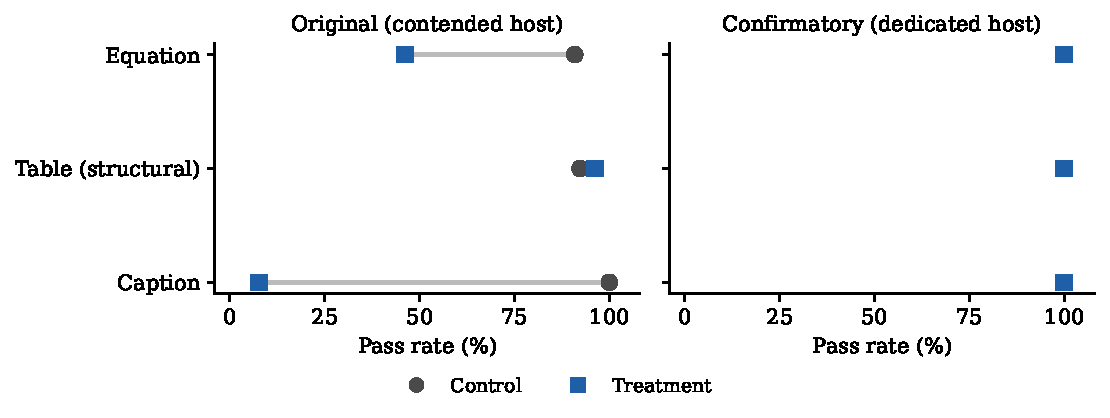
\includegraphics[width=\textwidth]{figures/fig-rendergate-dumbbell.pdf}
\caption{Control and treatment pass rates for the three write-time-verified families, original
contended host versus confirmatory dedicated host. The gap for equation and caption -- large on
the original host -- closes completely on the dedicated host; table-structural, already close on
the original host, closes the remainder.}
\label{fig:rendergate}
\end{figure}

\paragraph{Interpreting caption's originally significant gap.} Table~\ref{tab:render-gate}'s
paired test for caption returned $p<0.001$ on the original host, significant by the same test as
Section~\ref{sec:section-reorder}'s headline result. We do not read the two the same way.
Section~\ref{sec:section-reorder}'s finding measures whether an agent, given a chance to attempt a
task, does it correctly; here, treatment's write-time verification step instead declines to
persist a change at all whenever it cannot confirm correctness under the host conditions of the
moment, which is a gap in \emph{how often the arm successfully persists a change}, not in
\emph{whether a persisted change is correct}. This distinction makes a specific, falsifiable
prediction: removing host contention should close the gap. It does -- on a dedicated host,
caption's treatment reaches the identical 100\% as its control ($p=1.0$), confirming the
verification-reliability reading over a capability-limitation one.

\section{Ten real defects found and fixed}
\label{sec:defects}

The reported numbers depend on the harness, evaluator, and infrastructure that produced them, and
several of the defects below materially changed an already-reported number. We disclose each
rather than fold it silently into a final figure.

\begin{enumerate}
\item \textbf{Missing type-library cache broke basic Word COM (Component Object Model)
  automation.} The benchmark harness's write-time verification step falls back to Microsoft
  Word's own COM automation interface when the primary renderer is unavailable. Every real
  trial's temp-directory isolation (itself a fix for an earlier concurrency defect) incidentally
  emptied this cache on every trial, causing a plain dynamic-dispatch COM call to return an
  object missing basic properties. We fixed this by switching to an explicit type-library-bound
  dispatch call; verified live against the real COM backend, not a mock.
\item \textbf{A COM message-queue starvation bug.} Calling the file-save operation immediately
  after opening a document via COM could deterministically raise a
  ``call rejected by callee'' COM error -- confirmed non-transient via five consecutive failed
  retries with a real delay between each. We fixed this by explicitly servicing the COM message
  queue before the save call; it succeeded on the first attempt after the fix.
\item \textbf{The confirmatory harness discarded genuinely successful runs.} A changed output
  file on a trial killed by the harness's own outer timeout is safe, positive evidence the
  underlying edit had genuinely succeeded, because the write-time verification step is atomic:
  it restores the original file on any failure and only ever persists a change after independent
  verification succeeds. The harness did not act on that evidence -- whenever the wrapping
  process running a trial was killed, it unconditionally recorded that trial as failed, without
  ever checking what the verification step had actually left on disk. We fixed the harness to
  attempt grading in that case too, directly recovering two genuinely correct table-insertion
  trials, confirmed by re-grading the real output files against their own pre-write backups, not
  by re-running anything.
\item \textbf{A stale file-path bug after unrelated hardware disruption.} An external drive
  holding the benchmark's run data physically disconnected and reconnected under a different
  drive letter mid-project. The corpus manifest's document paths were still hardcoded to the
  old letter, causing every subsequent trial to fail on a permission error before it could even
  begin, rather than a clean not-found. We fixed this by correcting every path in the manifest.
\item \textbf{A transient network/certificate failure, not a capability finding.} We
  systematically reviewed every remaining trial's exact failure signature -- return code,
  whether the process timed out, whether the output file changed -- and found a signature not
  previously characterized: 29 trials across two families (equation, caption) failed with an
  API-level certificate verification error, not a timeout or a genuine grading failure. All 29
  clustered tightly in one short real-time window coinciding with the same unrelated hardware
  disruption in item 4, and the API's certificate was confirmed to verify correctly again
  immediately afterward. We re-ran these 29 trials under confirmed-healthy network conditions
  rather than counting them as capability failures: equation ultimately recovered from 4/26 to
  12/26 and caption from 1/26 to 2/26 (Table~\ref{tab:render-gate}, across several subsequent
  retry rounds -- see Section~\ref{sec:render-gate} for the full account, including a physically
  unreliable drive found along the way that this item's own retries first exposed). Before this
  item, Table~\ref{tab:render-gate}'s numbers for these two families had silently included these
  29 as ordinary capability failures -- a disclosure/reporting inconsistency corrected here and
  in that table.
\item \textbf{Two further evaluation-harness defects} -- an inverse-trial paragraph-id
  resolution bug affecting the citation family, and a statistics-regeneration gap that left a
  stale number published after an unrelated fix -- are described in full in the project's own
  working notes (\texttt{docs/} in the repository below) and omitted here for space.
\item \textbf{Sequential backend fallback could cost more time than the harness's own outer
  budget allowed.} The write-time verification step's two backends (Section~\ref{sec:render-gate})
  were tried sequentially, each with its own retry-bounded 90-second timeout -- discovering that
  both failed could cost up to their combined worst case (approximately 360 seconds), over half
  the harness's 600-second outer per-trial timeout. We fixed this by racing both backends
  concurrently instead, so discovering a double failure costs at most the slower of the two
  (approximately 180 seconds) rather than their sum. We are explicit that this changes latency
  under contention, not the underlying success probability: directly investigating this host's
  resource consumption while implementing this fix found a large, unrelated, CPU- and
  memory-heavy background workload (423\% CPU, 11.3GB resident memory) genuinely needed by its
  owner and left running -- both backends are starved by the same real resource shortage
  regardless of whether they are raced or chained, so this fix stops trials from being silently
  killed by the outer timeout mid-verification, but does not raise equation's or caption's pass
  rate.
\item \textbf{The confirmatory re-run's CLI silently refused every trial identically, and the
  failure signature was checked directly rather than assumed.} The first attempt at the
  dedicated-host confirmatory re-run (Section~\ref{sec:methods-rerun}) reported every one of 156
  chains as blocked, each in well under one second -- fast and uniform enough that we
  distrusted an infrastructure explanation on sight (a real host- or network-level failure is
  rarely both instant and perfectly uniform across three unrelated task families and both arms).
  Inspecting one chain's raw process output directly rather than guessing found the actual cause:
  the CLI invoked by every trial refuses to bypass its own permission checks when run as the
  root user, a deliberate safety restriction, and the cloud instance's default account is root.
  We fixed this by creating a dedicated non-root account for the re-run, verified functionally
  before re-running anything at scale, and confirmed the fix by re-inspecting individual trials'
  wall time and grading output (not merely their exit status) for realistic, varied values before
  trusting the run's aggregate numbers. This defect's exposure is a clean, fully-counted bound, not
  an open-ended risk: exactly 156 of 156 attempted chains failed this way before the fix, all 156
  were re-run after it, and none failed partially or silently in between.
\item \textbf{Every reported 100\%/0\% confidence interval was a bootstrap artifact.}
  \texttt{graph\_scorer.py}'s \texttt{bootstrap\_ci} function resamples only from the observed
  per-document pass/fail values; when every value is identical (a literal 100\% or 0\% observed
  rate), every possible resample is also identical to the original sample, so the percentile
  method has no source of variability and collapses to a zero-width $[100,100]$ interval --
  reporting no uncertainty at all rather than a real one, silently, on every boundary row in this
  paper (12 of them: Tables~\ref{tab:single-edit}, \ref{tab:render-gate}, and
  \ref{tab:render-gate-clean}). This was found while comparing this paper's statistical reporting
  against related empirical-reproducibility work, not by a user report or a test failure -- the
  existing unit test suite had encoded the degenerate behavior as the expected one. Fixed by
  falling back to the exact Clopper-Pearson interval specifically when the bootstrap resample
  distribution has zero variance (only possible at a literal 100\% or 0\% observed rate for
  binary data); every other row's interval is untouched, since the ordinary percentile bootstrap
  is not degenerate away from that boundary. The corrected intervals are visibly wider and
  honestly represent less certainty than $[100,100]$ implied -- e.g., 26/26 passes now reports
  $[86.8, 100]$, not $[100,100]$ -- without changing a single point-estimate pass rate anywhere in
  this paper.
\end{enumerate}

Every defect above was independently re-verified against real output data -- either by
re-running the affected trial live, or by re-deriving the grading verdict directly from the
already-collected output file -- rather than assumed fixed once the code changed.

\section{Discussion}
\label{sec:discussion}

This benchmark's central capability finding is that bounded structural tools resist the state
drift a generic-tool agent shows under repeated edit-undo cycling. This result is more
informative than any single-edit pass-rate comparison, because it isolates a mechanism -- fresh
anchor resolution versus accumulated agent-maintained state -- rather than reporting an aggregate
number. We expect this mechanism to generalize to any repeated-editing workflow, not just section
reordering specifically, though this benchmark tests only one task family at depth.

The write-time-verification-gated families illustrate a different, under-discussed methodological
hazard: an architectural choice made for a good reason (never persist a corrupt document) can
produce a benchmark result that looks like a capability finding but is substantially a
deployment-environment artifact. Disentangling the two required real, disclosed engineering work
(Section~\ref{sec:defects}) and a controlled confirmatory re-run (Section~\ref{sec:methods-rerun}),
not just a larger sample size or a more careful argument. Rejecting the most obvious alternative
explanation -- that these tools are simply more expensive to render-verify than table
insertion's -- was not sufficient on its own; the attribution to shared-host contention and a
physically unreliable test-host component required a direct test, not an inference. Re-running
the identical benchmark on a dedicated, single-tenant host closed the gap completely for both
equation and caption (Table~\ref{tab:render-gate-clean}). The general lesson extends past this
specific benchmark: a write-time verification step's reported reliability is only as meaningful
as the host it was measured on, and a benchmark result that looks like a capability finding is
worth testing against a change of deployment environment before it is reported as one.

\section{Limitations and threats to validity}
\label{sec:limitations}

Seven factors limit generalization. \textbf{First}, this benchmark tests only
the \texttt{claude-sonnet-5} model and does not claim the results generalize across models.
\textbf{Second}, the write-time-verification-gated families' originally-reported numbers
(Table~\ref{tab:render-gate}) were collected on a single, shared, variably-contended host rather
than a dedicated one, and that host condition materially depressed two of the three families'
numbers -- confirmed, not merely argued, by the confirmatory re-run in
Table~\ref{tab:render-gate-clean}, which closes the gap completely on a dedicated host. We
therefore treat Table~\ref{tab:render-gate-clean} as the load-bearing result for these three
families and Table~\ref{tab:render-gate} as evidence for the host-contention claim rather than as
a competing final number. This resolution does not extend past this specific verification
mechanism: we make no claim that shared-host contention is never a genuine factor for other
write-time-verification designs, only that it fully explains the gap observed here.
\textbf{Third}, corpus size for section reordering ($n=11$ at $K=1$ on the original corpus) is
small before the follow-up corpus is combined in. \textbf{Fourth}, one specific piece of our own
test infrastructure -- an external drive holding all run data -- proved physically unreliable,
disconnecting twice during this project (confirmed via OS-level disk I/O error events, not
inferred); this remains a real defect in our original test environment (Section~\ref{sec:defects}),
though the confirmatory re-run's clean result means it is no longer load-bearing for any number
in this paper's final reporting. \textbf{Fifth}, this benchmark exercises 11 of Meridian Docs'
86 registered tools, across the six families reported here; the remaining tools -- other editing
operations, format/style-compliance audit tools such as \texttt{audit\_document} and
\texttt{audit\_equation\_style}, and read-only structural/indexing tools including
\texttt{locate\_anchor} and \texttt{index\_document} -- are outside this benchmark's scope, and we
do not claim these results generalize to the full tool surface. Relatedly, every trial reported
here receives its target anchor pre-resolved at corpus-build time (Section~\ref{sec:methods});
the live anchor-resolution tools' own reliability under real, uncontrolled use is a real question this
benchmark does not measure -- their content-derived synthetic ids are explicitly documented as
shifting if an earlier paragraph with the same text is edited, inserted, or removed elsewhere in
the document. \textbf{Sixth}, this corpus is not a blind holdout in the machine-learning sense:
several defects (Section~\ref{sec:defects}) were found by observing trial outcomes on this same
26-document corpus during the benchmark's own execution, then fixed directly in the tooling and
the affected chains re-run (Section~\ref{sec:methods}). We mitigate, but do not eliminate, the
resulting risk in two ways that distinguish this from conditioning a statistical model on its own
test set: every fix targets a deterministic code defect (a wrong file path, a schema-invalid
element order), not the underlying language model's prompts, weights, or grading criteria, which
never varied; and every fix was independently re-verified against real re-run data rather than
assumed effective. We do not claim these numbers estimate performance on documents this tooling
has never previously encountered in any form. \textbf{Seventh}, the per-trial subprocess timeout
(300s, 600s for the render-gated families) was not derived from an expected-task-duration
analysis (Section~\ref{sec:methods}); a genuinely slow but correct chain on either arm could in
principle be misclassified as an infrastructure exclusion rather than allowed to finish.

\subsection{Artifact availability}
This benchmark's harness, evaluator, statistics code, and corpus manifests are publicly available
at \url{https://github.com/ajc3xc/ooxml-graph-paper} under the MIT license. The underlying
\texttt{.docx} corpus documents themselves are a licensed slice of the DocOps benchmark corpus
and are not redistributed; the released manifests identify which documents were used (by hash)
without including their content.

\section{Conclusion}
\label{sec:conclusion}

Bounded, structurally-aware editing primitives like Meridian Docs show no advantage over generic
file tools for a single document edit, on the task families and model tested here, but show a significant,
mechanistically-traced advantage under repeated editing -- the more realistic condition for an
agent maintaining a document over time. Three further task families were initially confounded by
a write-time verification step whose reliability cost proved substantial and
environment-dependent; a controlled confirmatory re-run on a dedicated, single-tenant host
resolved that confound completely, closing all three families to 100\% pass for both arms and
confirming the original gap was a deployment-environment artifact rather than an editing-capability
limitation. We report both the original and confirmatory numbers, and the live infrastructure
work connecting them, rather than reporting a single clean number that would understate how much
of this benchmark's own execution environment turned out to matter.

\textbf{Future work.} Whether audit-style tools like \texttt{audit\_document} and
\texttt{audit\_equation\_style} (Section~\ref{sec:limitations}) help an agent bring a document
into compliance with a target venue's formatting guidelines is a natural next question, but not
one this benchmark's methodology can answer as-is: unlike the six families reported here,
guideline compliance has no single deterministic ground truth. Grading it would need a rubric
built from two sources together -- a venue's own published guidelines for its unambiguous rules
(margins, citation style), and a real accepted paper from that venue to resolve the guidelines'
vaguer clauses -- evaluated with the same treatment-versus-control design used throughout this
paper, not an ablation in place of one. A small, exploratory pilot along these lines already
exists: four fixtures, \texttt{audit\_equation\_style} versus generic tools, reported in full in
our internal notes rather than here. Both arms matched on three hand-authored fixtures, but the
one real, organically-occurring document tested surfaced a genuine, previously-unknown bug in the
audit tool itself that only the unbounded control arm caught. Too small a sample to support any
claim -- but a concrete argument for running this at confirmatory scale, not a reason to treat the
question as settled either way.

\todo{This is a preliminary draft. Before any submission: (1) re-run a full writing-quality and
content-quality review against this revision, since the most recent pass (which added the
research questions, the Clopper-Pearson defect/fix, the artifact-availability link, and the
expanded Related Work below) has not itself been re-reviewed; (2) decide a target venue --
ACM REP (the Conference on Reproducibility and Replicability) is the leading candidate given
this paper's confirmatory framing and defect-disclosure emphasis, per its own CFP -- and convert
from this generic-article format to that venue's actual template and page limit.}

\bibliographystyle{plainnat}
\bibliography{refs}

\end{document}
